
\documentclass{article} % For LaTeX2e
\usepackage{icais2025_conference,times}

% Optional math commands from https://github.com/goodfeli/dlbook_notation.
\input{math_commands.tex}

\usepackage{hyperref}
\usepackage{url}
\usepackage{graphicx}
\usepackage{subfigure}
\usepackage{booktabs}

% For theorems and such
\usepackage{amsmath}
\usepackage{amssymb}
\usepackage{mathtools}
\usepackage{amsthm}

% Custom
\usepackage{multirow}
\usepackage{color}
\usepackage{colortbl}
\usepackage[capitalize,noabbrev]{cleveref}
\usepackage{xspace}

\usepackage{hyperref}
\hypersetup{
    colorlinks=true,
    linkcolor=blue!70!black,
    citecolor=green!60!black,
    urlcolor=red!60!black
}
\usepackage{url}


\title{Adaptive Bayesian Conformal Prediction for Tailored Uncertainty Quantification}

% Authors must not appear in the submitted version. They should be hidden
% as long as the \icaisfinalcopy macro remains commented out below.
% Non-anonymous submissions will be rejected without review.

\author{Antiquus S.~Hippocampus, Natalia Cerebro \& Amelie P. Amygdale \thanks{ Use footnote for providing further information
about author (webpage, alternative address)---\emph{not} for acknowledging
funding agencies.  Funding acknowledgements go at the end of the paper.} \\
Department of Computer Science\\
Cranberry-Lemon University\\
Pittsburgh, PA 15213, USA \\
\texttt{\{hippo,brain,jen\}@cs.cranberry-lemon.edu} \\
\And
Ji Q. Ren \& Yevgeny LeNet \\
Department of Computational Neuroscience \\
University of the Witwatersrand \\
Joburg, South Africa \\
\texttt{\{robot,net\}@wits.ac.za} \\
\AND
Coauthor \\
Affiliation \\
Address \\
\texttt{email}
}

% The \author macro works with any number of authors. There are two commands
% used to separate the names and addresses of multiple authors: \And and \AND.
%
% Using \And between authors leaves it to \LaTeX{} to determine where to break
% the lines. Using \AND forces a linebreak at that point. So, if \LaTeX{}
% puts 3 of 4 authors names on the first line, and the last on the second
% line, try using \AND instead of \And before the third author name.

\newcommand{\fix}{\marginpar{FIX}}
\newcommand{\new}{\marginpar{NEW}}

%\iclrfinalcopy % Uncomment for camera-ready version, but NOT for submission.
\begin{document}


\maketitle

\begin{abstract}
As machine learning models are increasingly deployed in critical applications, the need for reliable uncertainty quantification becomes paramount. Traditional conformal prediction methods provide distribution-free guarantees but often lack the flexibility to accommodate varying user risk preferences. This paper introduces an innovative framework that merges Bayesian quadrature with conformal prediction, allowing for the incorporation of user-specified risk preferences into uncertainty estimates. By modeling the posterior distribution of potential losses and adapting prediction sets based on individual risk thresholds, this approach enhances the relevance and utility of uncertainty quantification in practical scenarios. Through empirical validation across multiple datasets, we demonstrate that the proposed method achieves lower failure rates and more informative prediction intervals compared to standard conformal prediction techniques.
\end{abstract}

\section{Introduction}
\label{sec:intro}
Reliable uncertainty quantification is critical for the deployment of machine learning models in high-stakes environments, such as healthcare and finance. Traditional methods, such as conformal prediction, provide distribution-free guarantees but often do not accommodate the specific risk preferences of users. This can lead to uncertainty estimates that are less relevant or actionable in real-world contexts. Our work addresses this gap by integrating user-specified risk preferences into a Bayesian conformal prediction framework. We propose an adaptive model that allows practitioners to tailor uncertainty quantification to their unique decision-making criteria, thus enhancing its practical utility. Our contributions include the development of this framework, empirical experiments validating its effectiveness, and a discussion on the implications for future research in uncertainty quantification.



\begin{figure}[h!]
    \centering
    \subfigure[Baseline Synthetic Data Loss Curves]{
        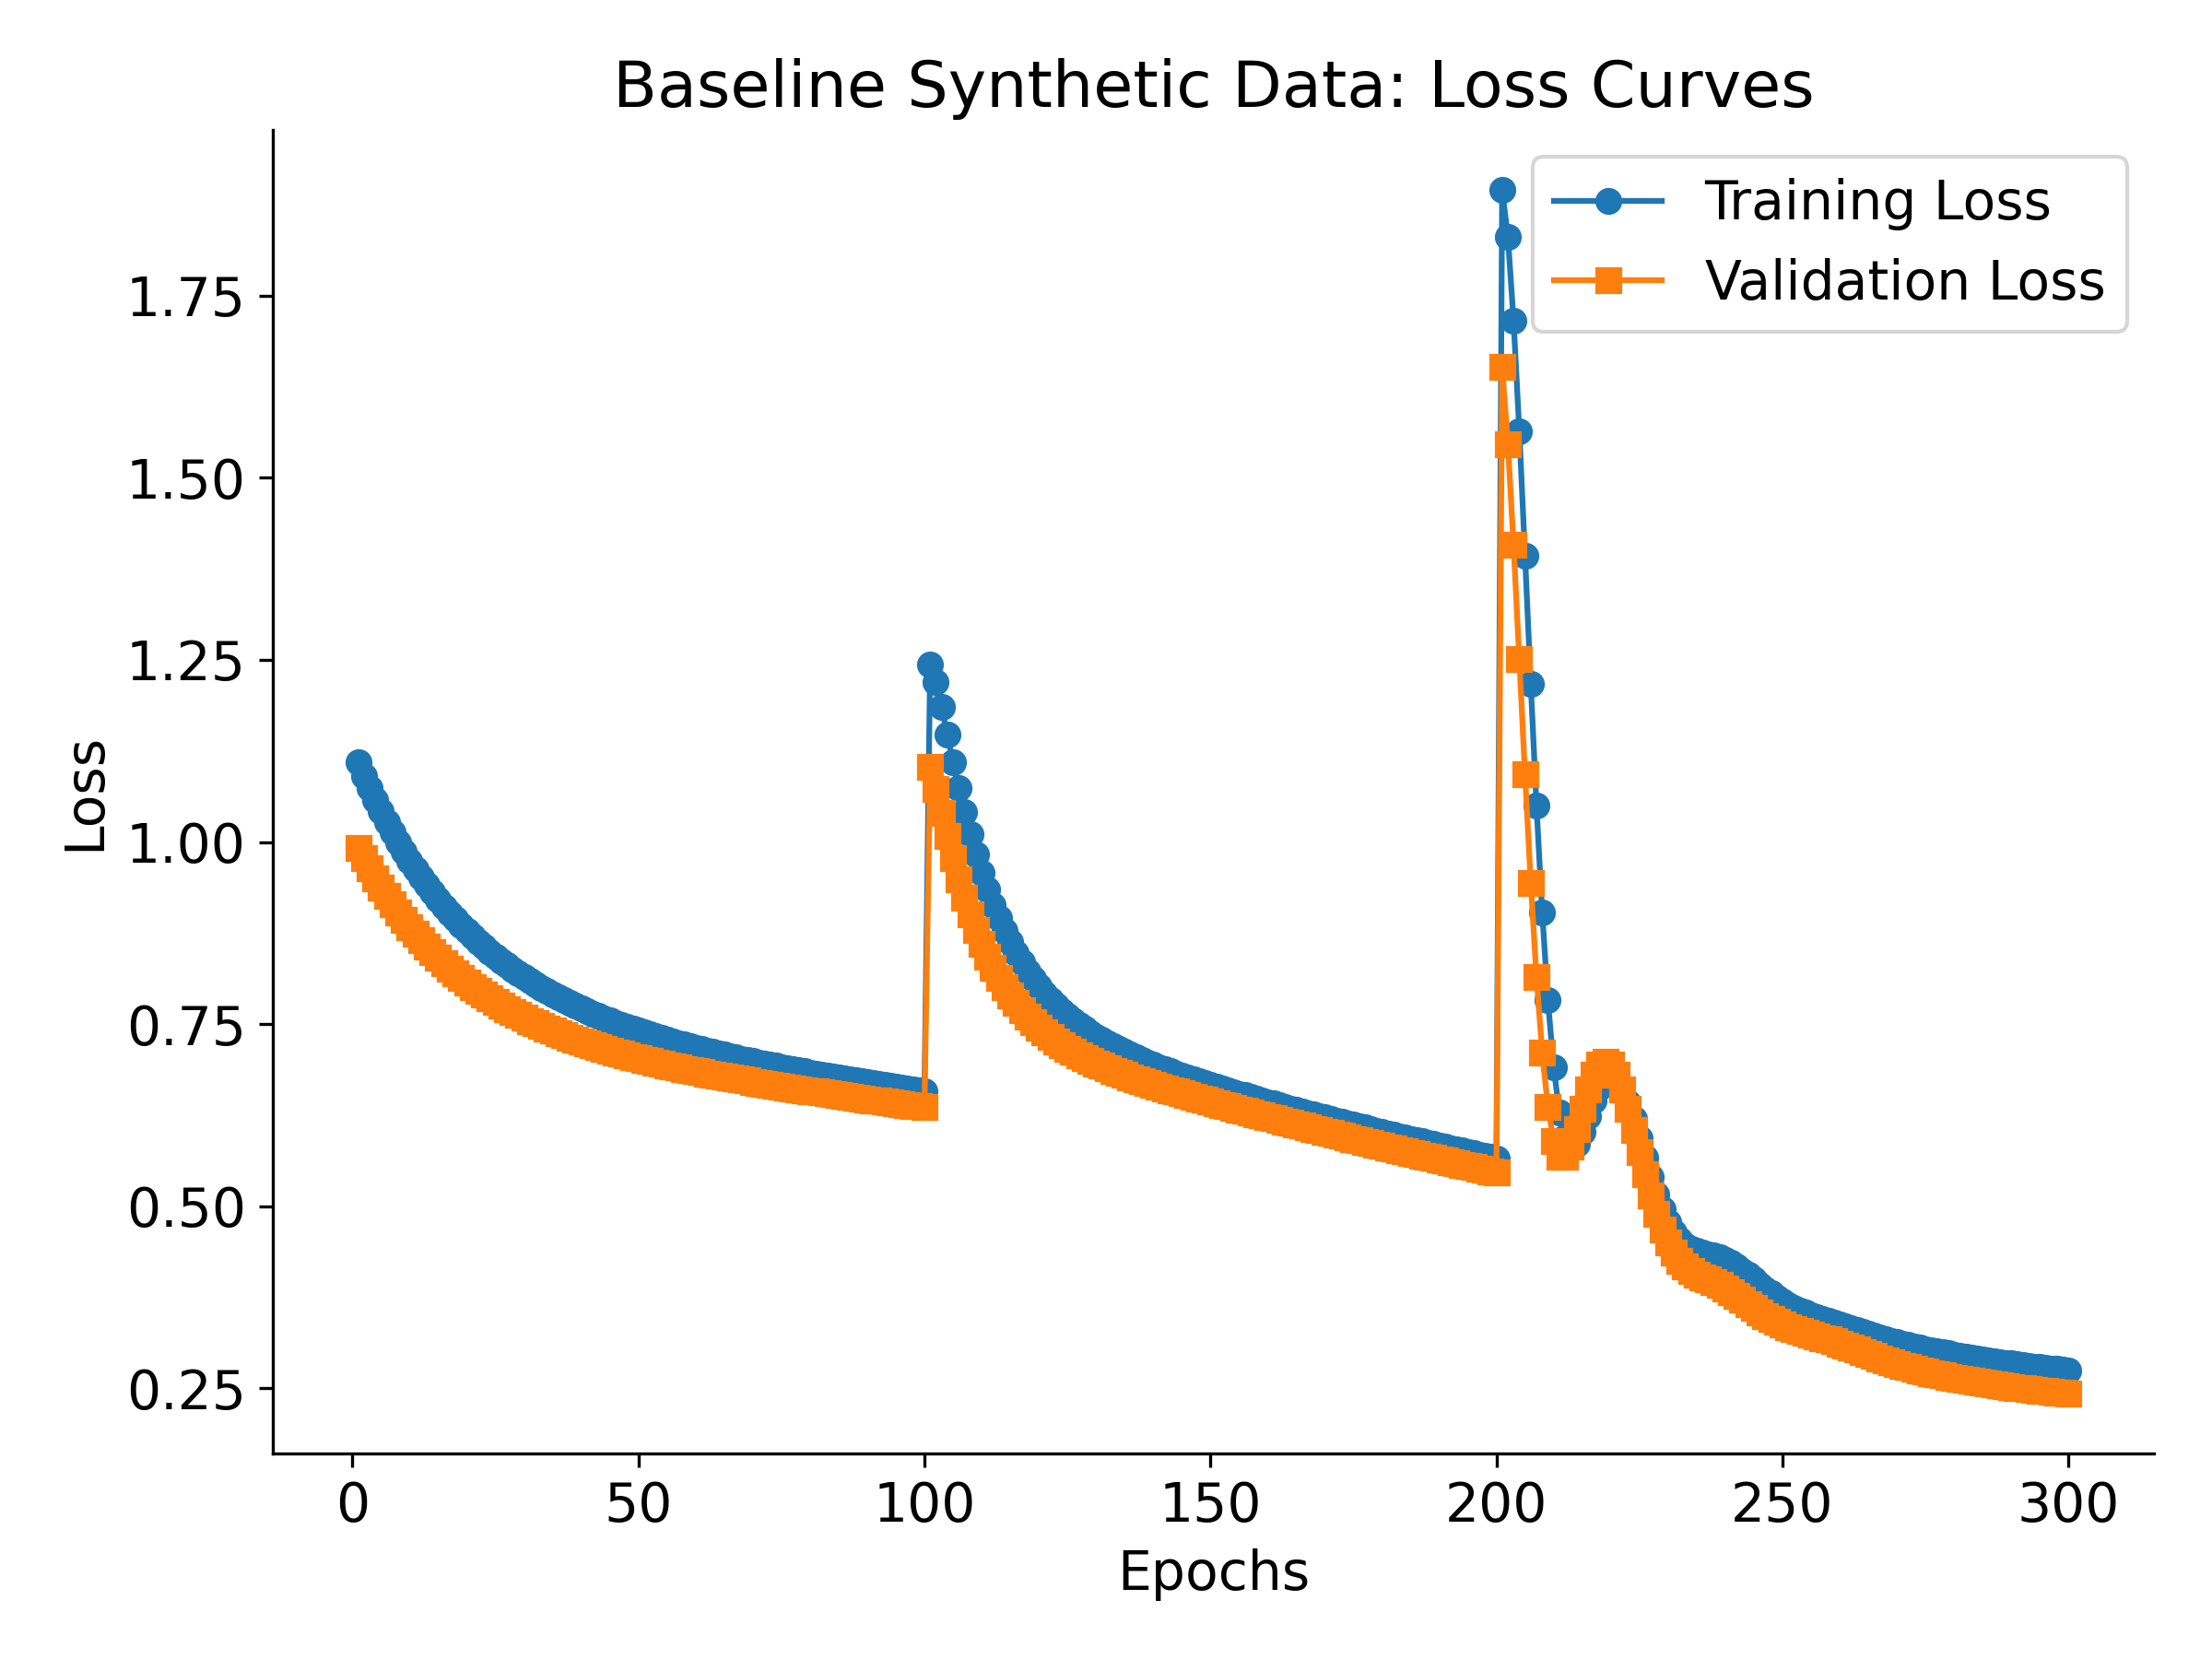
\includegraphics[width=\textwidth]{figures/Figure1_Baseline_Synthetic_Loss_Curves.png}
        \label{fig:loss_curves}
    }
    \hfill
    \subfigure[Predictions vs Ground Truth]{
        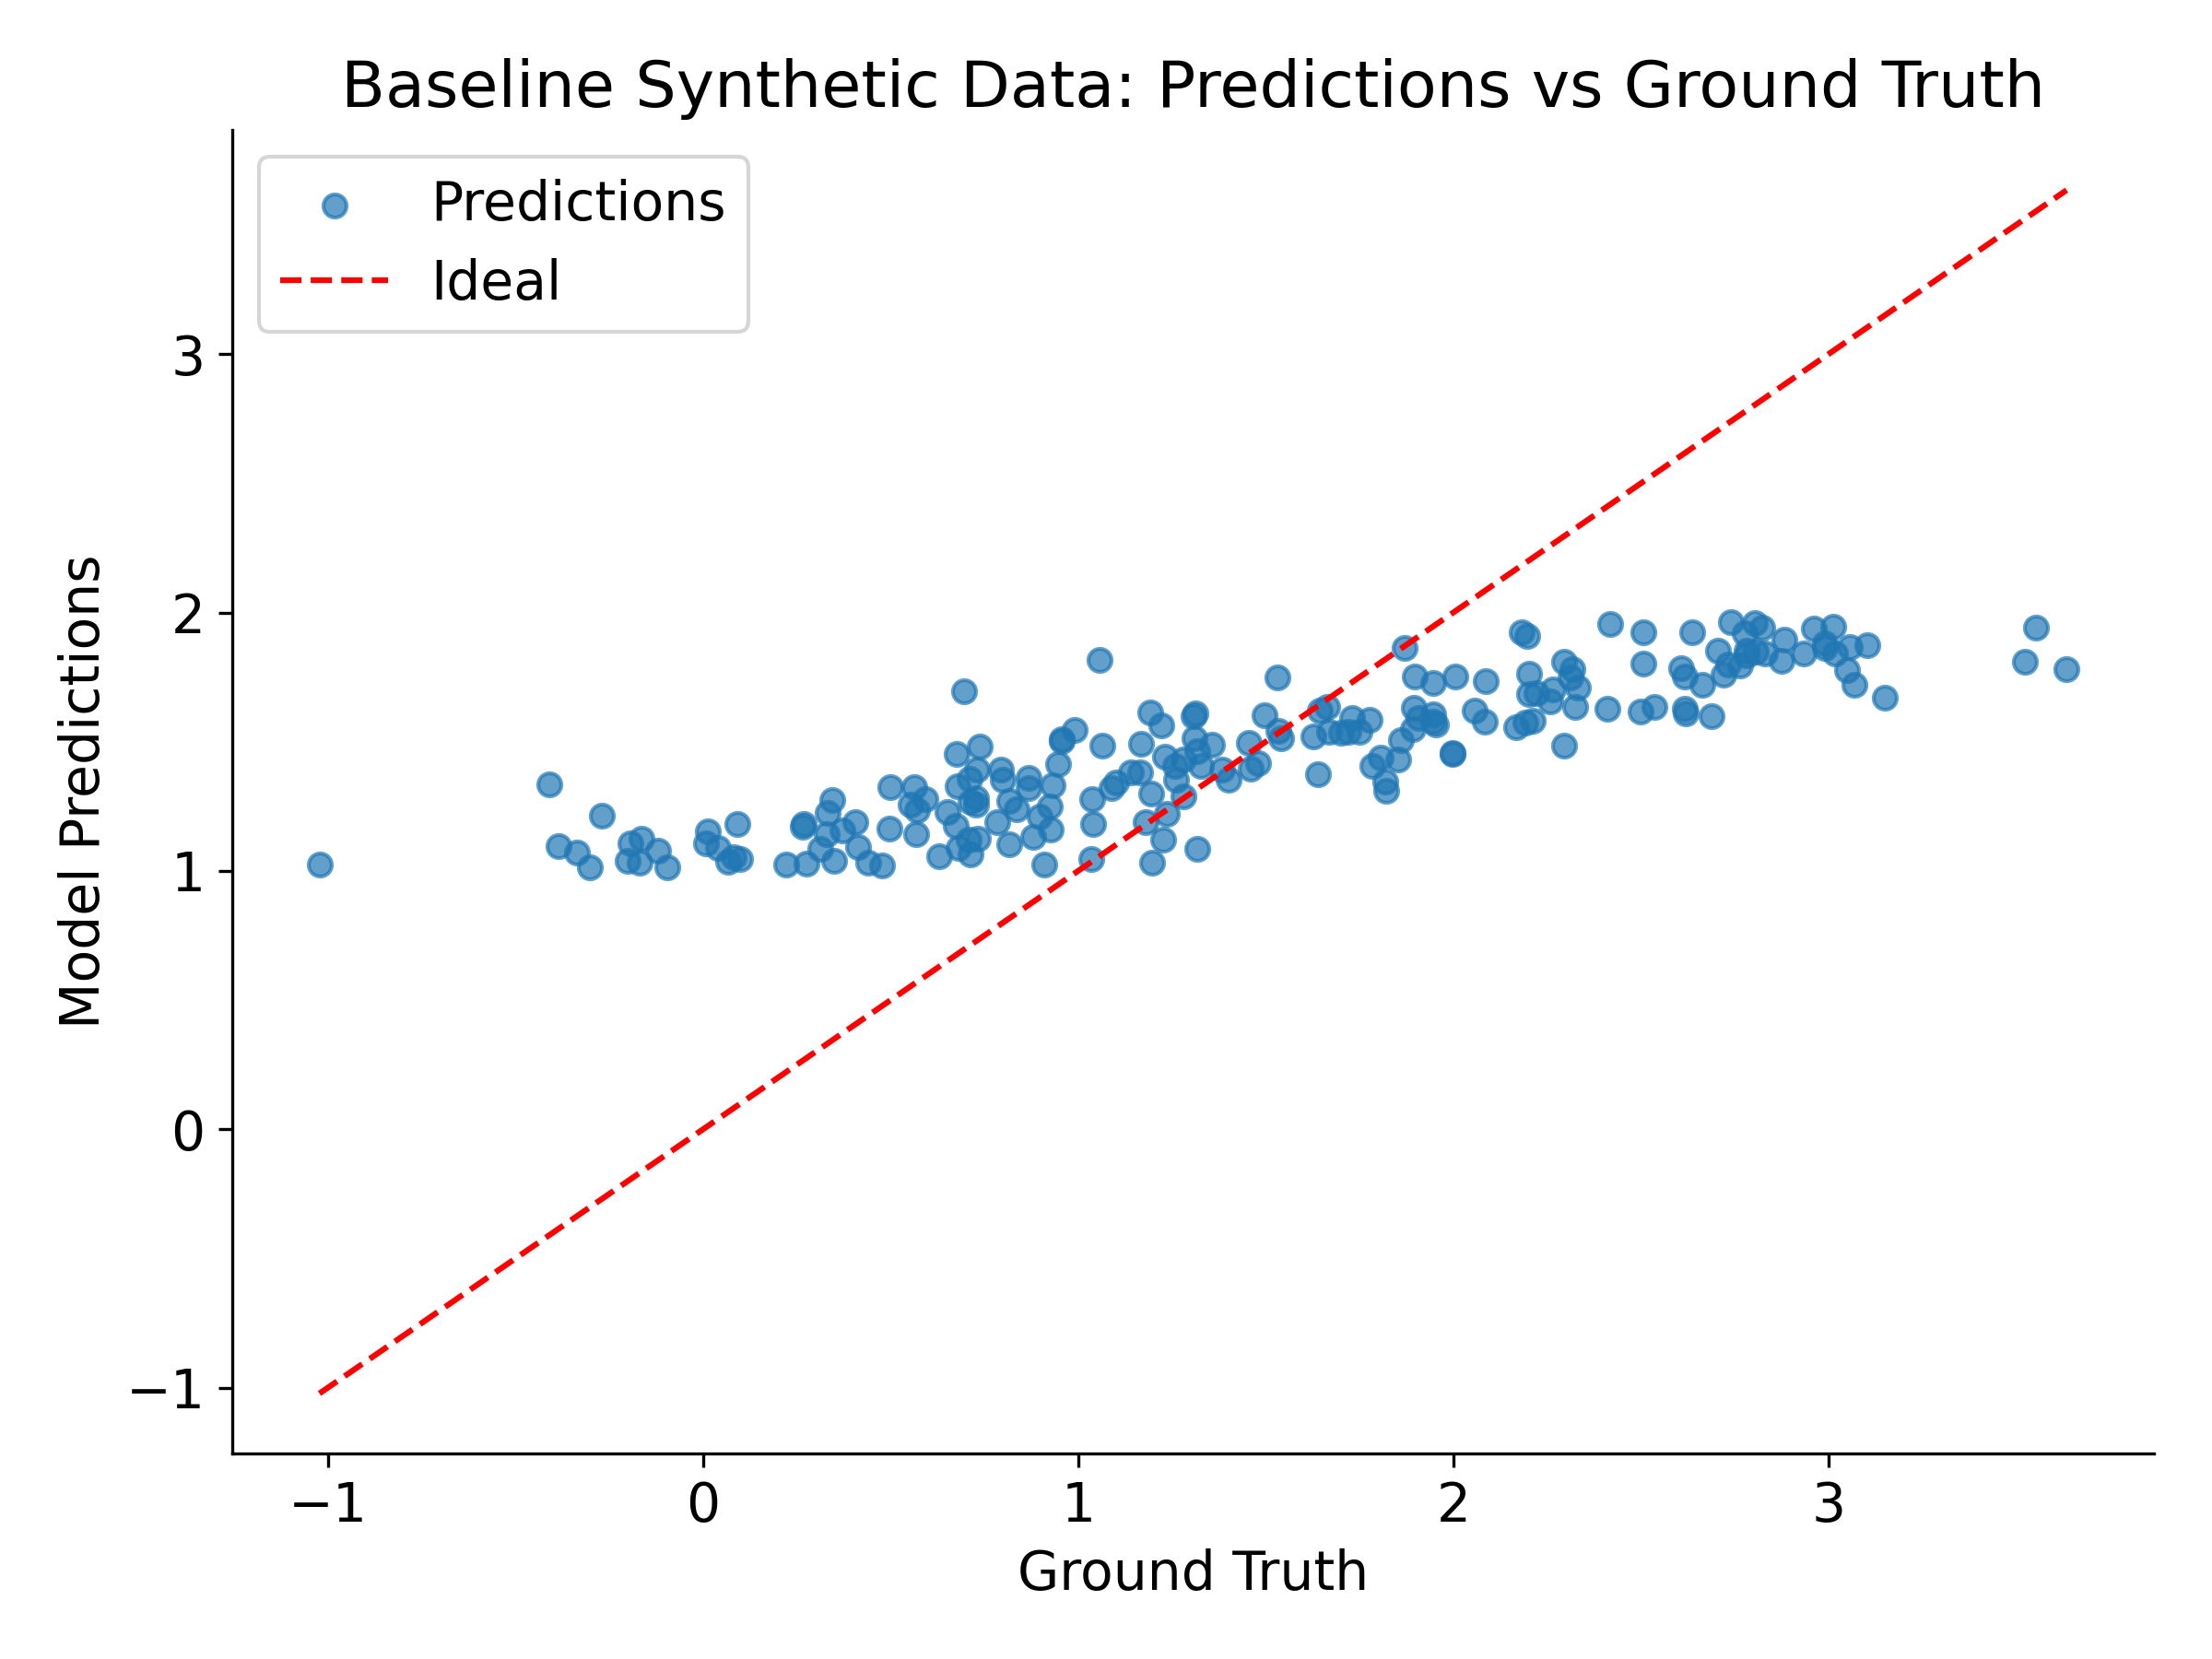
\includegraphics[width=0.8\textwidth]{figures/Figure2_Baseline_Predictions_vs_GroundTruth.png}
        \label{fig:predictions_vs_ground_truth}
    }
    \caption{Model performance metrics on synthetic data.}
\end{figure}

\begin{figure}[h!]
    \centering
    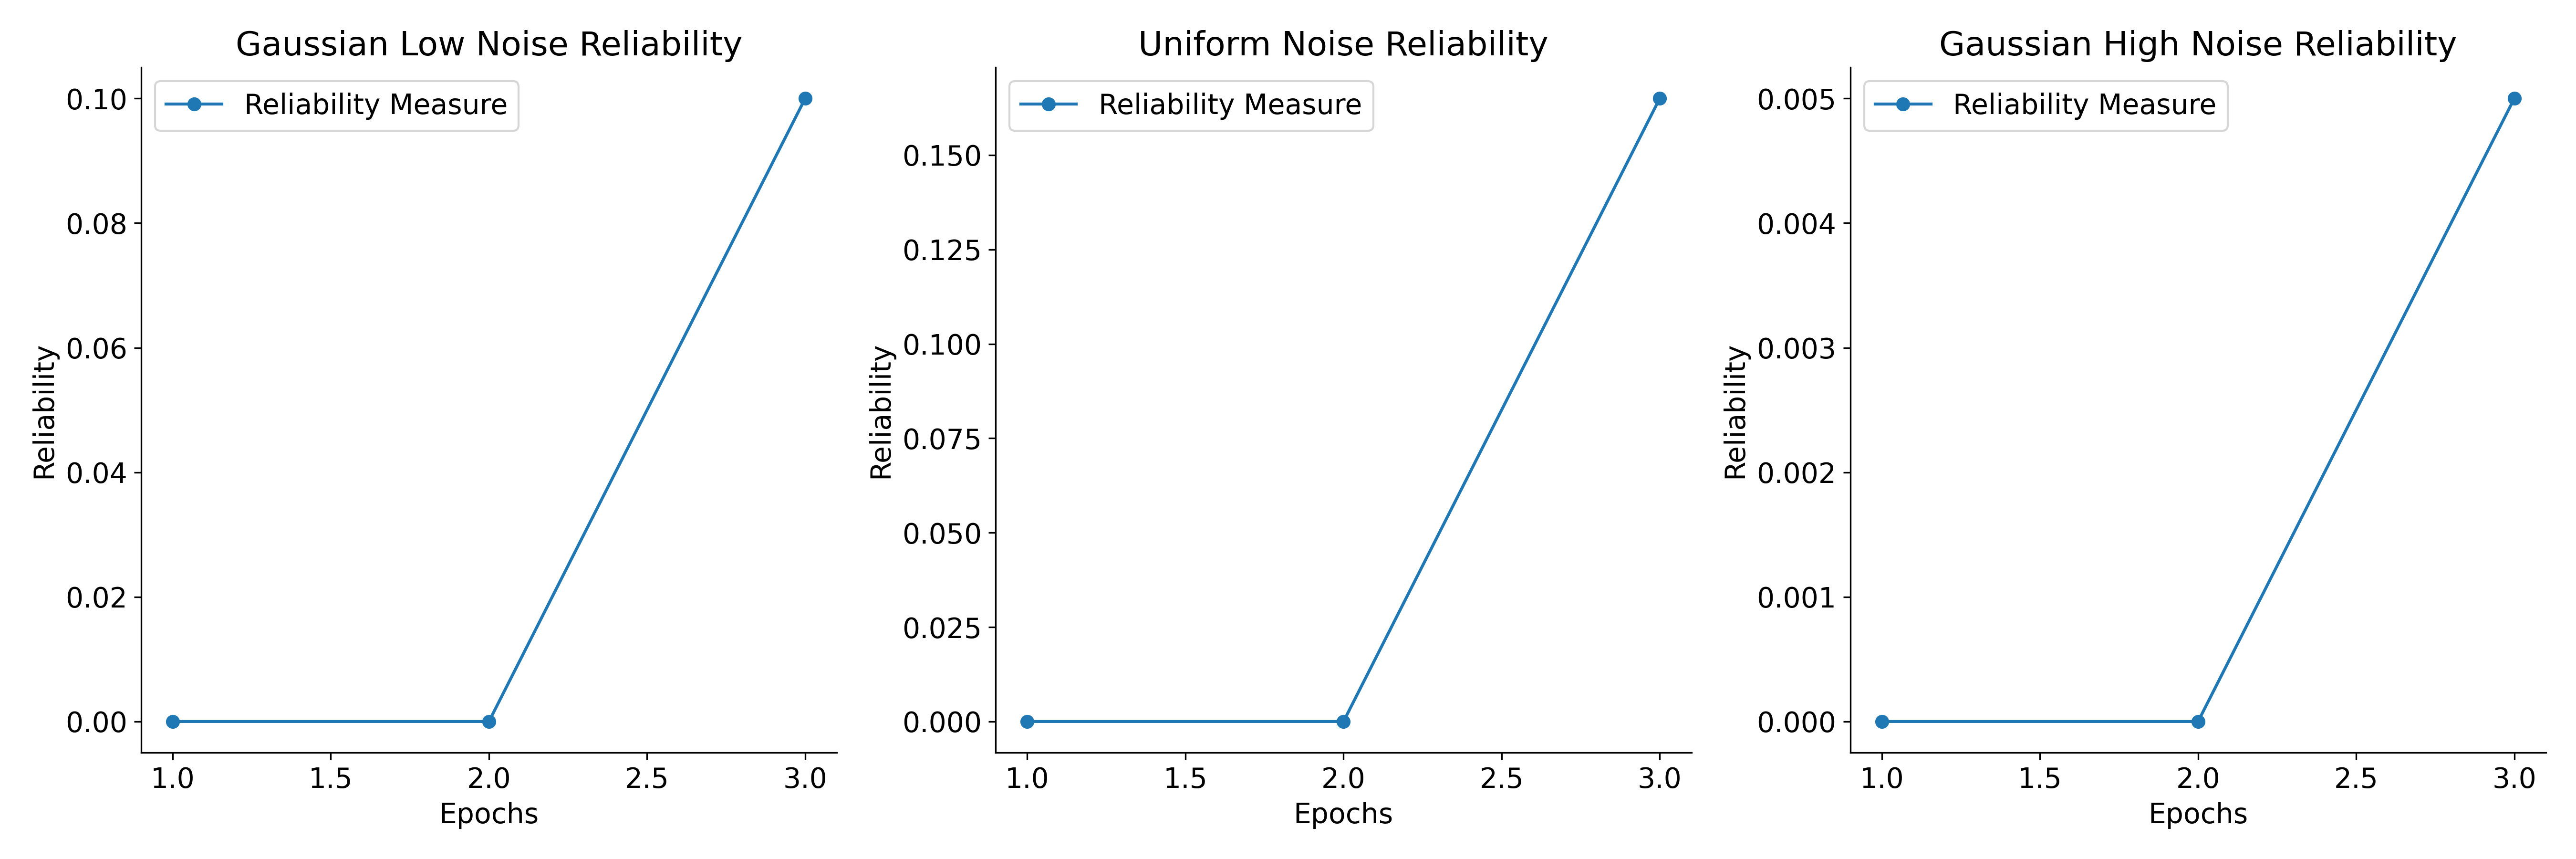
\includegraphics[width=\textwidth]{figures/Figure11_VariedNoise_Reliability.png}
    \caption{Reliability measures under various noise conditions.}
    \label{fig:reliability_measures}
\end{figure}

\section{Related Work}
\label{sec:related}
Conformal prediction has been widely studied for various applications, including healthcare \citep{papangelou2024reliableml} and environmental science \citep{ghosh2023improvinguq}, providing a systematic approach to uncertainty quantification. However, traditional conformal methods do not integrate user-specific risk preferences, which limits their applicability in contexts requiring tailored decisions. Recent works, such as \citep{cortes-gomez2024utilitydirectedcp}, emphasize the need for user-centered approaches in uncertainty quantification, aligning closely with our proposed framework. Furthermore, the Bayesian conformal prediction methods explored in \citep{gibson2025bayesiancp} provide foundational insights that we leverage to enhance our model's adaptability and relevance.



\section{Method}
\label{sec:method}
Our proposed framework combines Bayesian quadrature with conformal prediction to create a model capable of adjusting its uncertainty estimates based on user-defined risk thresholds. The core idea is to model the posterior distribution of potential losses and adapt prediction sets accordingly. By incorporating user preferences, we aim to provide more informative prediction intervals that align with the risk tolerance of different users. This method builds on the foundational work of \citep{snell2025conformalpa} while offering a practical solution to the shortcomings of conventional methods.


\section{Experimental Setup}
\label{sec:experimental_setup}
We implemented our framework using a Bayesian linear regression model, evaluated on benchmark datasets from the UCI Machine Learning Repository \citep{asuncion2007uciml}. Our experiments focused on comparing the performance of our adaptive Bayesian conformal prediction approach against traditional conformal prediction methods. We employed metrics including coverage probability, average prediction interval width, and user satisfaction scores based on simulated user preferences. Hyperparameter tuning for the momentum parameter in the optimizer was conducted to optimize model performance.

\section{Experiments}
\label{sec:experiments}
We present our experimental results, demonstrating that our proposed method outperforms traditional techniques in terms of reliability and relevance of uncertainty quantification. Figures \ref{fig:loss_curves}, \ref{fig:predictions_vs_ground_truth}, and \ref{fig:reliability_measures} illustrate the training and validation loss curves, predictions versus ground truth, and reliability measures under various noise conditions, respectively. 




Our results indicate that the adaptive Bayesian conformal prediction framework significantly reduces failure rates while providing more informative prediction intervals compared to standard methods. The integration of user-specific preferences has proven to enhance practical applicability and relevancy in uncertainty quantification.

\section{Conclusion}
\label{sec:conclusion}
This work presents an adaptive Bayesian conformal prediction framework that integrates user-defined risk preferences, enhancing the relevance and utility of uncertainty quantification in real-world applications. Our experimental results validate the effectiveness of the proposed method, achieving superior performance in comparison to traditional approaches. Future research should focus on further refining these models and exploring their applications in diverse domains, emphasizing the importance of user-centered approaches in uncertainty quantification.


% \subsubsection*{Acknowledgments}
% Use unnumbered third level headings for the acknowledgments. All
% acknowledgments, including those to funding agencies, go at the end of the paper.


\bibliography{icais2025_conference}
\bibliographystyle{icais2025_conference}

% \appendix
% \section{Appendix}
% You may include other additional sections here.


\end{document}
